\documentclass{beamer}
\usepackage[utf8]{inputenc}
\usepackage{graphicx}
\usepackage{listings}
\usepackage{hyperref}
\hypersetup{
	colorlinks=true,
	linkcolor=blue,
	filecolor=magenta,      
	urlcolor=cyan,
}

\urlstyle{same}

\usepackage{xcolor}

\lstdefinestyle{base}{
	language=C++,
	emptylines=1,
	breaklines=true,
	basicstyle=\ttfamily\color{black},
	moredelim=**[is][\bf\color{red}]{@}{@},
}

\usetheme[]{boxes}
\usecolortheme{seagull}
\addtobeamertemplate{navigation symbols}{}{%
	\usebeamerfont{footline}%
	\usebeamercolor[fg]{footline}%
	\hspace{2em}%
	\insertframenumber/\inserttotalframenumber
}

%\usepackage{french}
\title{Modèles et techniques en programmation parallèle hybride et multi-c\oe urs}
\subtitle{Parall\'elisme multithreads (2)}
\author{Marc Tajchman}\institute{CEA - DEN/DM2S/STMF/LMES}
\date{10/08/2020}

\begin{document}
\begin{frame}
	\titlepage
\end{frame}

\large
\begin{frame}
	\section{Techniques de programmation avec OpenMP}
	\frametitle{Techniques de programmation avec OpenMP}

\begin{itemize}
	\item Programmation OpenMP grain fin
	\bigskip
	\item Programmation OpenMP grain grossier
	\bigskip
	\item Programmation OpenMP par tâches
\end{itemize}
\end{frame}

\begin{frame}[fragile]
	\frametitle{Programmation OpenMP de type ``grain fin''}
	
	Cela consiste à ajouter un pragma devant les boucles à paralléliser pour que OpenMP découpe automatiquement l'ensemble de valeurs de l'indice de boucle en groupes.
	
	\vfill
	Chaque thread prend en charge un des groupes. Chaque groupe est (à peu près) de même taille (en nombre d'itérations).
	\vfill
	
	Par exemple:
	
\lstset{%
	language={C++},
	breaklines=true,
	captionpos=b,
	basicstyle=\ttfamily,
	moredelim=[il][\color{red}]{/+},%
}

\begin{lstlisting}{C++}
   /+#pragma omp parallel for
   for (i=0; i<n; i++)
     u[i] = f(a, v[i]);
\end{lstlisting}
	
		
	\vfill
	Le programmeur a assez peu de possibilités pour adapter la répartition à un problème particulier
\end{frame}


\begin{frame}
	Avantages~:
	\begin{itemize}
		\item Simple à programmer (si la boucle est simple).
		
		\item La différence entre le code parallèle et le code séquentiel est l'ajout de pragmas, donc on peut garder une seule version des sources.
		
		\item On peut paralléliser progressivement un code, choisir les boucles à paralléliser.
	\end{itemize}

\vfill

	Désavantages~:
	\begin{itemize}
		\item Les régions parallèles sont souvent plus nombreuses et plus petites, ce qui décroît souvent les performances.
		\item La répartition est équilibrée en nombre d'itérations pas en temps calcul, souvent certains threads ont fini avant les autres et sont inemployés.
		\item Les boucles complexes sont plus difficiles ou impossibles à paralléliser (boucles ``while", boucles sur des indices non entiers, etc.)
	\end{itemize}
\end{frame}

\begin{frame}[fragile]
	Soit l'algorithme suivant: on part d'une valeur initiale de $u$ et on calcule une suite de $nT$ valeurs de $u$ pour $t > 0$.
	
	\lstset{%
		language={C++},
		breaklines=true,
		captionpos=b,
		basicstyle=\ttfamily,
		moredelim=[il][\color{red}]{/+},%
	}
	
	\begin{lstlisting}{C++}
for (iT=0; iT < nT; iT++)
{
  dT = calcul_dt(u);
  for (iX=1; iX < nX-1; iX++)
    v[iX] = f(u[iX-1],u[iX],u[iX+1],dT)
  echange(u, v);
}
	\end{lstlisting}
	
	\vfill
	La boucle externe (sur \verb|iT|) n'est pas parallélisable
	\begin{itemize}
		\item chaque itération modifie le même vecteur $v$,
		\item chaque itération dépend de toutes les précédentes.
	\end{itemize}
\end{frame}

\begin{frame}[fragile]
Pour paralléliser, il ne reste que la boucle interne (sur \verb|iX|):

\lstset{%
	language={C++},
	breaklines=true,
	captionpos=b,
	basicstyle=\ttfamily,
    numbers=left,
    numbersep=5pt,
    numberstyle=\tiny\color{gray},
    rulecolor=\color{black},
    showspaces=false,
    showstringspaces=false,
	moredelim=[il][\color{red}]{/+},%
}

\begin{lstlisting}{C++}
for (iT=0; iT < nT; iT++)
{
  dT = calcul_dt(u);
  /+#pragma omp parallel for
  for (iX=0; iX < nX; iX++)
    v[iX]=f(u[iX-1],u[iX],u[iX+1],dT);
  echange(u, v);
}
\end{lstlisting}

\vfill
Il y a donc {\bf nT régions parallèles} (avec création des threads à l'entrée - ligne 14 - et destruction des threads à la sortie - après la ligne 16).
\vfill
\end{frame}

\begin{frame}[fragile]
	\frametitle{Programmation OpenMP de type ``grain grossier''}

\vfill
Cela consiste à :
\medskip

\begin{itemize}
	\item 
	essayer de définir des régions parallèles plus grandes et moins nombreuses.
\vfill

\begin{quote}
	Cela conduit souvent à des régions parallèles dans lesquelles une partie des instructions ne sont pas exécutées par tous les threads (utilisation des pragmas \textcolor{red}{\tt single} et \textcolor{red}{\tt master}, ou des indices de threads : {\tt omp\_get\_thread\_num()}).
\end{quote}

	\item découper soi-même les boucles internes pour mieux tenir compte de la différence de temps calcul entre les itérations.
\end{itemize}

\vfill
\end{frame}

\begin{frame}
	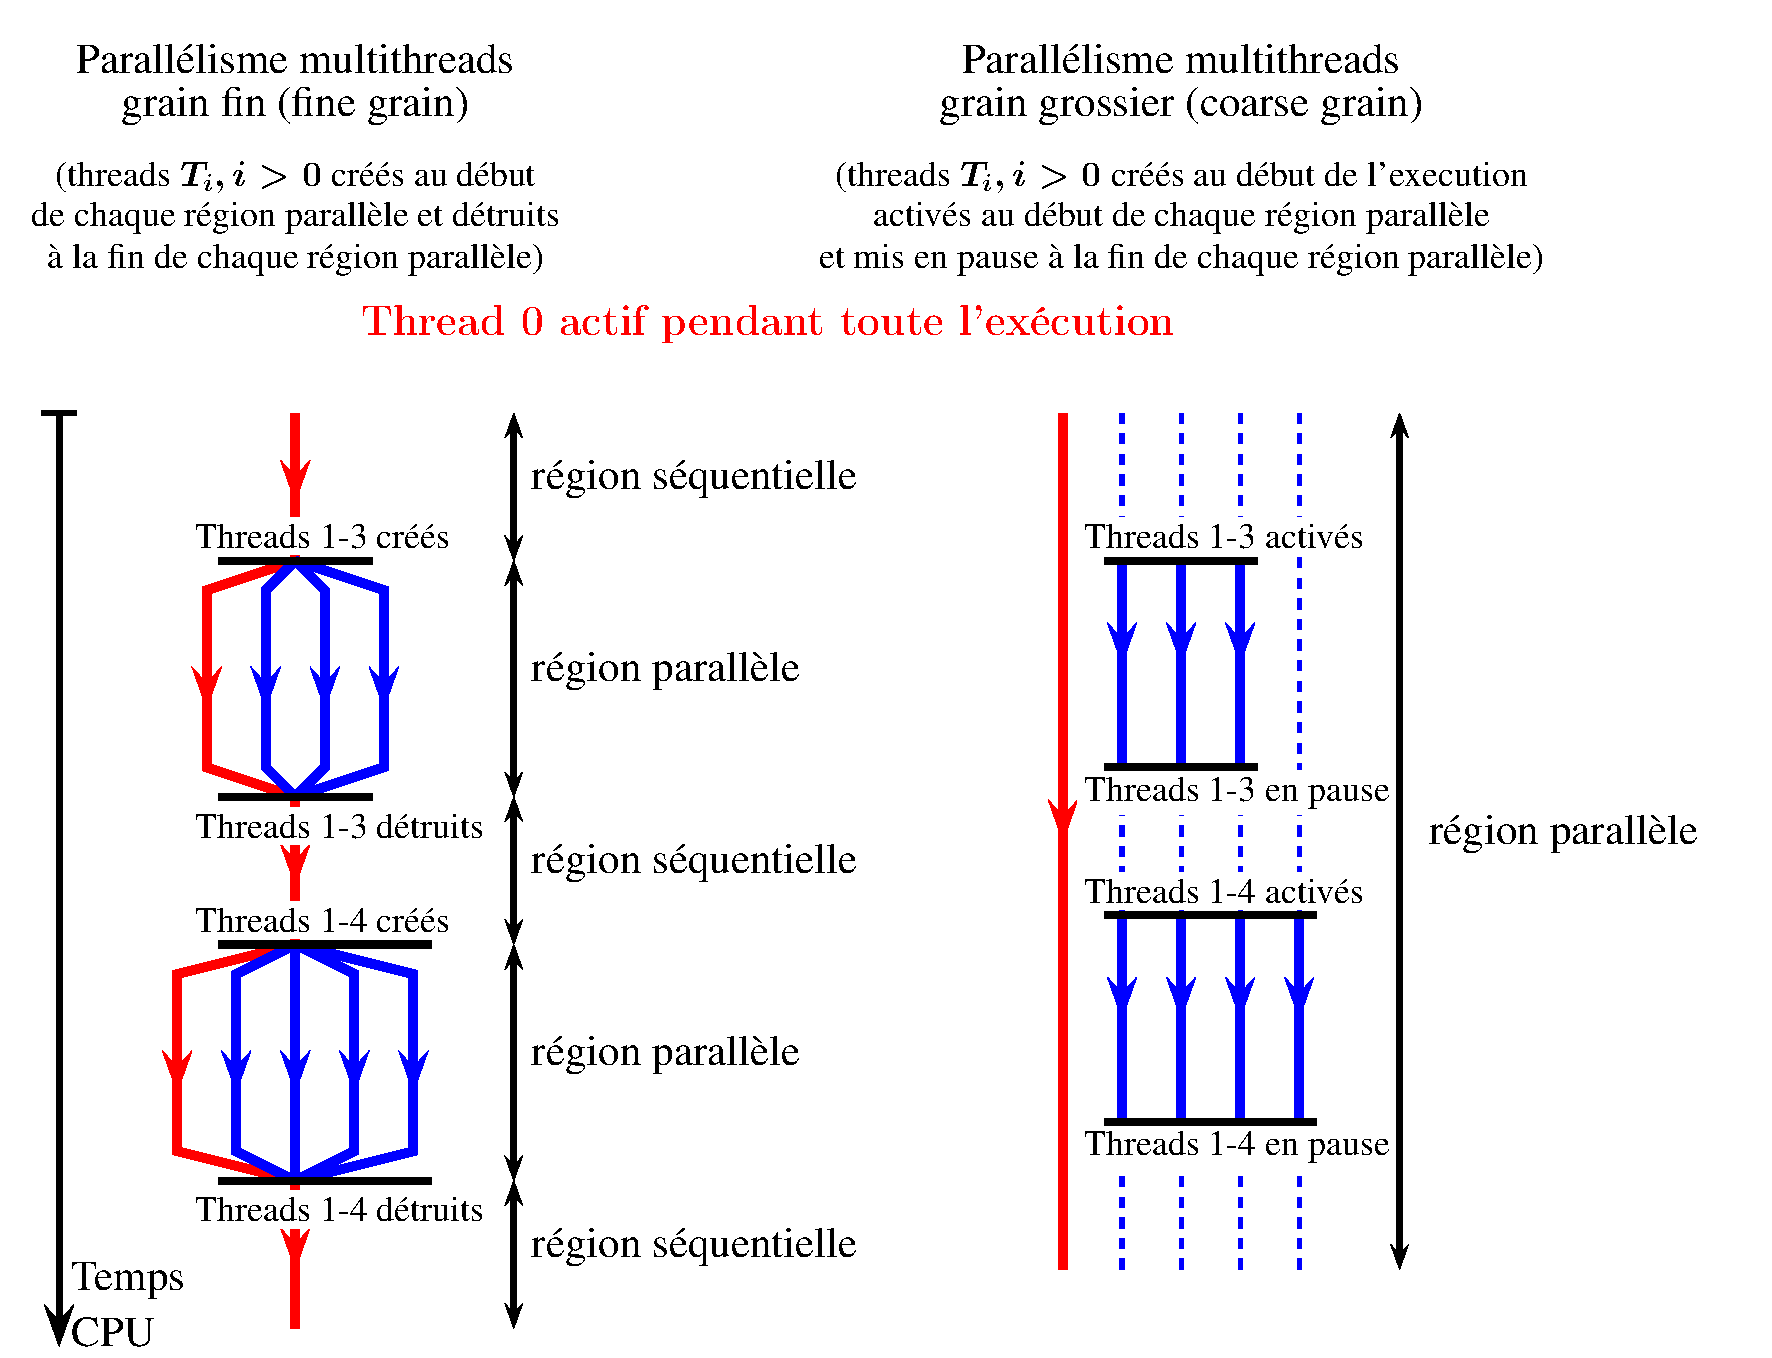
\includegraphics[scale=0.40]{../../Images/enchainement_coarse}
\end{frame}

\begin{frame}[fragile]
	\textcolor{blue}{Illustration du premier point : on crée une seule région parallèle}
	
	\lstset{%
		language={C++},
		breaklines=true,
		captionpos=b,
		basicstyle=\ttfamily,
        firstnumber      = 1,
        numbers=left,
        numbersep=5pt,
        numberstyle=\tiny\color{gray},
		moredelim=[il][\color{red}]{/+},%
	}
	
	\begin{lstlisting}{C++}
/+#pragma omp parallel default(shared)
{
  int iT, iX;
  for (iT=0; iT < nT; iT++)
  {
    /+#pragma omp single
    dT = calcul_dt(u);
    
    /+#pragma omp for
    for (iX=1; iX < nX-1; iX++)
      v[iX] = f(u[iX-1],u[iX],u[iX+1],dT)

    /+#pragma omp single
    echange(u, v);
  }
}
\end{lstlisting}
	
\vfill
\end{frame}

\begin{frame}[fragile]
	\textcolor{blue}{Illustration du second point : on définit soi-même le découpage de la boucle interne}
	
	\lstset{%
		language={C++},
		breaklines=true,
		captionpos=b,
		basicstyle=\ttfamily,
		moredelim=[il][\color{red}]{/+},%
	}
	
	\begin{lstlisting}{C++}
#pragma omp parallel default(shared)
{
  int iT, iX;
  /+int iTh = omp_get_thread_num();
  /+int nTh = omp_get_num_threads();
  /+int d = nX/nTh;
  /+int nX1 = iTh*d;
  /+int nX2 = n1 + d; if(iTh==nTh-1)nX2=nX; 
  for (iT=0; iT < nT; iT++)
  {
    #pragma omp single
    dT = calcul_dt(u);
    /+for (iX=nX1; iX < nX2; iX++)
      v[iX] = f(u[iX-1],u[iX],u[iX+1],dT)
    #pragma omp single
    echange(u, v);
  }
}
	\end{lstlisting}
	
	\vfill
\end{frame}

\begin{frame}
    \vfill
	Avantages~:
	\begin{itemize}
		\item On crée moins de régions parallèles (une seule dans l'exemple).
		\item Le découpage de la boucle interne est fait une seule fois et c'est le développeur qui détermine ce découpage.
	\end{itemize}

    \vfill
    Suivant le type de problème, la programmation à grain grossier pourra être plus ou moins intéressante.
    
    \vfill
	Désavantages~:
    \begin{itemize}
    	\item L'écriture du code est plus complexe (savoir quand mettre en pause certains threads par exemple).
    	\item Il est moins facile de maintenir un source unique pour les versions séquentielle et parallèle.
   \end{itemize} 
    \vfill
    
\end{frame}

\begin{frame}[fragile]
	\frametitle{Programmation OpenMP par tâches}

On définit dans le codes des groupes d'instructions qui peuvent être exécutés en parallèle, qu'on appelle ``tâches''. 
\vfill

Il peut y avoir un nombre de tâches différent du nombre de threads (en général, il y aura plus de tâches que de threads).
\vfill
 
Quand les tâches sont définies, le système les met dans une file d'attente. Les tâches sont exécutées dès qu'un c\oe ur est disponible.
\vfill
Avantages : 
\begin{itemize}
	\item On peut définir un nombre de tâches inconnu à l'avance (boucle ``while'' par exemple).
	\item Une tâche peut elle-même créer d'autres tâches (parallélisme à plusieurs niveaux).
\end{itemize}
Inconvénient : 
\begin{itemize}
	\item On ne sait pas exactement quand une tâche sera lancée, ce qui rend délicat la gestion des variables partagées.
\end{itemize}
\end{frame}

\begin{frame}[fragile]
Exemple : Calcul de la suite de Fibonacci définie par la récurrence
$$
F_n = F_{n-1} + F_{n-2}
$$
avec $F_0 = 0$ et $F_1 = 1$.

\vfill
Exemple de code en C/C++ (fonction récursive):
 
	\lstset{%
	language={C++},
	captionpos=b,
	basicstyle=\ttfamily
}

\begin{lstlisting}{C++}
long f(int n)
{
  if (n<2)
    return n;
  else
    return f(n-1) + f(n-2);
}
\end{lstlisting}

\end{frame}

\begin{frame}[fragile]
\vfill
	On peut remarquer que :
	\begin{itemize}
		\item dans $f$, découpage du travail seulement en 2 parties
		\item $f$ est récursive, donc si on utilise des pragma dans $f$, elles seront utilisées de façon récursive
	\end{itemize}

\bigskip
Le nombre de threads utilisés peut rapidement dépasser le nombre de c\oe urs disponibles, ce qui est assez compliqué à gérer.
\vfill
\end{frame}

\begin{frame}[fragile]
	Première version utilisant des sections OpenMP
	
\begin{lstlisting}{C++}
long f(int n) {
  if (n < 2) return n;
  long a, b;
  
  omp_set_num_threads(2)
#pragma omp parallel sections
  {
  #pragma omp section
    a = f(n-1);		
  #pragma omp section
    b = f(n-2);
  }
  return a + b;
}
\end{lstlisting}

\vspace{-2cm}\hfill\framebox{\begin{minipage}{6cm}
Cette version va créer $2^L$ threads où $L$ est le nombre de niveaux de récursivité.
\end{minipage}
}
\end{frame}

\begin{frame}
	\vfill

	Voir {\tt\textcolor{blue}{Exemples3/omp\_sections}}.
	\vfill
	
	L'exemple fonctionne relativement bien, mais l'utilisation des sections a 2 désavantages:
	
	\begin{itemize}
		\item Le nombre de sections est fixe pour chaque niveau de parallélisation.
		\item Il faut bien utiliser la fonction {\tt\textcolor{blue}{omp\_set\_num\_threads}} sinon risque ``d'étouffer'' la machine
	\end{itemize}

	\vfill
\end{frame}

\begin{frame}[fragile]
	Seconde version utilisant les tâches OpenMP:
	
	
\begin{lstlisting}{C++}
long fib_tasks(int n) {
	
  long i, j;
  if (n<2)
    return n;

#pragma omp task shared(i, n)
  i=fib_tasks(n-1);
#pragma omp task shared(j, n)
  j=fib_tasks(n-2);
		
#pragma omp taskwait
		
  return i+j;
}
\end{lstlisting}

\end{frame}

\begin{frame}
	
\vfill

Voir {\tt\textcolor{blue}{Exemples3/omp\_tasks}}.

\vfill
Cette version utilisant les tâches OpenMP permet d'enlever les désavantages des sections et de, plus, on peut contrôler le nombre total de threads utilisé par le code.

\vfill
Mais:
\begin{itemize}
	\item Faire attention au nombre de tâches créées (2 à la puissance $n$).

	En pratique on met une limite au nombre de niveaux de récursivité.
	
\vfill
	\item Utiliser les résultats d'une tâche seulement quand on est sûr que la tâche est terminée : pas de barrière implicite à la fin de {\tt omp task}
	
	Donc, il faut appeler {\tt omp taskwait} avant d'utiliser {\tt i} ou {\tt j} (pour calculer {\tt i+j}).
\end{itemize}

\end{frame}

\begin{frame}
	Le répertoire \textcolor{blue}{Exemples3/sinus} contient 5 sous-répertoires
	qui tous comparent deux méthodes de calcul de $y=sin(x)$, soit par la fonction système soit une approximation par une formule de Taylor.
	\medskip
	
	Remarque: on a artificiellement ralenti le calcul de la formule de Taylor pour mieux faire ressortir les temps de calcul.
	
	\begin{itemize}
		\item \textcolor{blue}{sinus\_seq}: calcul séquentiel
		\item \textcolor{blue}{sinus\_omp\_fine\_grain}: calcul OpenMP grain fin
		\item \textcolor{blue}{sinus\_omp\_coarse\_grain}: calcul OpenMP grain grossier
		\item \textcolor{blue}{sinus\_omp\_adaptatif}: calcul OpenMP grain grossier avec équilibrage de charge
		\item \textcolor{blue}{sinus\_omp\_task}: calcul OpenMP par tâches
	\end{itemize}

\vfill

\end{frame}

\begin{frame}

Il existe plusieurs autres outils pour faire de la programmation multi-threads.
\bigskip

On commentera ici deux exemples qui utilisent 
\begin{itemize}
	\item{\tt std::thread} : similaires à pthread mais de style plus C++ et avec des mécanismes plus évolués
	\item {\tt tbb} : Threads Building Blocks, aussi spécifiques à C++ et plus souples, mais à installer séparemment
\end{itemize} 
\end{frame}

\begin{frame}
Exemple utilisant {\tt std::thread}, voir \textcolor{blue}{\tt Exemples3/std\_thread}
\bigskip

Commentaires
\end{frame}

\begin{frame}
Exemple utilisant {\tt tbb}, voir \textcolor{blue}{\tt Exemples3/tbb}
\bigskip

Commentaires
\end{frame}

\end{document}
